\documentclass[hyperref=unicode,utf8,xcolor=pst]{beamer}
\usetheme{boxes}
\setbeamertemplate{navigation symbols}{}
%
\definecolor{mirantisred}{RGB}{166,38,20}
\setbeamercolor{titlelike}{fg=mirantisred}
\setbeamercolor{structure}{fg=mirantisred}
%
\usepackage[T2A]{fontenc}
%
\usepackage{graphicx}
\usepackage{fancyvrb}
%
% Copyright (c) 2013  Mirantis, Inc.
%
%    Licensed under the Apache License, Version 2.0 (the "License"); you may
%    not use this file except in compliance with the License. You may obtain
%    a copy of the License at
%
%         http://www.apache.org/licenses/LICENSE-2.0
%
%    Unless required by applicable law or agreed to in writing, software
%    distributed under the License is distributed on an "AS IS" BASIS, WITHOUT
%    WARRANTIES OR CONDITIONS OF ANY KIND, either express or implied. See the
%    License for the specific language governing permissions and limitations
%    under the License.
%
\title{Ceph in Mirantis OpenStack}
%\author{
\includegraphics[height=4cm, trim=3cm 2cm -5cm 4cm, clip]{Vector_RGB_MirantisLogo}\\Dmitry Borodaenko}
\author{
\includegraphics[height=4.5cm]{Vector_RGB_MirantisLogo}\\Dmitry Borodaenko}
\date{Mountain View, 2013\\ Mirantis}
%
\begin{document}

\begin{frame}
	\titlepage
\end{frame}

\begin{frame}
	\setcounter{framenumber}{1}
	\frametitle{\insertframenumber{}. The Plan}
	\begin{enumerate}
		\item What is Ceph?
		\item How does Ceph fit into OpenStack?
		\item What can you make Ceph do with Fuel?
		\item Gotchas and limitations
		\item Ceph architecture overview
		\item Storage architecture for OpenStack with Ceph
		\item Deploying Ceph with Mirantis OpenStack
		\item Operating Ceph backed OpenStack services
		\item Troubleshooting
		\item Resources
	\end{enumerate}
\end{frame}

\begin{frame}
	\frametitle{\insertframenumber{}. What is Ceph?}
	Ceph is a free storage system that provides unified object,
	block, and file storage.

	\begin{description}
		\item[Object Storage] RADOS objects support
			snapshotting, replication, and consistency.
		\item[Block Storage] RBD block devices are thinly
			provisioned over RADOS objects and can be
			accessed by Qemu via librbd library.\\
			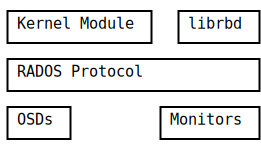
\includegraphics[height=3cm]{ceph-rbd}
		\item[File Storage] CephFS metadata servers (MDS)
			provide a POSIX-compliant overlay ovre RADOS.
	\end{description}
\end{frame}

\end{document}
